\documentclass[12pt]{article}
\usepackage{amsmath}
\usepackage{amssymb}
\usepackage[top = 1 in, bottom = 1 in, left = 1 in, right = 1 in]{geometry}
\usepackage{graphicx}
\usepackage{float}
\usepackage{cite}
\usepackage{bm}
\usepackage{url}
\usepackage{fancyvrb}
\usepackage{multirow}


\newcommand{\abs}[1]{\left| #1 \right|} % for absolute value
\newcommand{\avg}[1]{\left< #1 \right>} % for average
\newcommand{\prns}[1]{\left( #1 \right)} % for scaling parens
\newcommand{\brkt}[1]{\left[ #1 \right]} % for scaling brackets
\newcommand{\dgr}[0]{^\circ} % for degree
\newcommand{\ihat}[0]{ \hat{\imath}}
\newcommand{\jhat}[0]{ \hat{\jmath}}
\newcommand{\khat}[0]{ \hat{k}}
\newcommand{\N}[0]{\notag \\} % align endlines
\newcommand{\ket}[1]{\left| #1 \right>} % for Dirac bras
\newcommand{\bra}[1]{\left< #1 \right|} % for Dirac kets
\newcommand{\braket}[2]{\left< #1 \vphantom{#2} \right|
 \left. #2 \vphantom{#1} \right>} % for Dirac brackets
\newcommand{\spin}[2]{\begin{pmatrix} #1\\ #2\\\end{pmatrix}}
\newcommand{\sspin}[2]{\left( \begin{smallmatrix} #1 \\ #2 \end{smallmatrix} \right)}
\newcommand{\ntwo}[0]{ \frac{1}{\sqrt{2}}}
\newcommand{\degr}[0]{ ^\circ}


\usepackage[hang,small,bf]{caption}

\setlength\parindent{0pt}
\parskip 8pt

\title{ Hand Activity Recognition \\ Project Planning \\ UW Madison - HCI Lab }
\author{Ruisen (Eric) Liu}

\usepackage{graphicx}
%\begin{figure}[H]
%\begin{center}
%\includegraphics[trim = 35mm 95mm 40mm 90mm, clip, width=0.6\textwidth]{Case1_Theoretical.pdf}
%\caption{A plot of the analytical solutions for Case 1.}
%\end{center}
%\end{figure}

\usepackage{pdfpages}

\usepackage{fancyhdr}
\pagestyle{fancy}
\rhead{Eric Liu}
%\cfoot{Page \thepage}
\fancyfoot[C]{\thepage}

\usepackage{longtable}
\usepackage{tabularx}
%%%%%%%%%%%%%%%%%%%%%%%%%%%%%%%%%%%%%%%%%%%%%%%%%%%%%%
% For the Codes
\usepackage{listings}
\usepackage{color}

\definecolor{mygreen}{rgb}{0,0.6,0}
\definecolor{mygray}{rgb}{0.5,0.5,0.5}
\definecolor{mymauve}{rgb}{0.58,0,0.82}

\lstset{ %
  backgroundcolor=\color{white},   % choose the background color; you must add \usepackage{color} or \usepackage{xcolor}
  basicstyle=\footnotesize,        % the size of the fonts that are used for the code
  breakatwhitespace=false,         % sets if automatic breaks should only happen at whitespace
  breaklines=true,                 % sets automatic line breaking
  captionpos=b,                    % sets the caption-position to bottom
  commentstyle=\color{mygreen},    % comment style
  deletekeywords={...},            % if you want to delete keywords from the given language
  escapeinside={\%*}{*)},          % if you want to add LaTeX within your code
  extendedchars=true,              % lets you use non-ASCII characters; for 8-bits encodings only, does not work with UTF-8
  frame=single,                    % adds a frame around the code
  keepspaces=true,                 % keeps spaces in text, useful for keeping indentation of code (possibly needs columns=flexible)
  keywordstyle=\color{blue},       % keyword style
  language=C,                 % the language of the code
  morekeywords={*,...},            % if you want to add more keywords to the set
  numbers=left,                    % where to put the line-numbers; possible values are (none, left, right)
  numbersep=5pt,                   % how far the line-numbers are from the code
  numberstyle=\tiny\color{mygray}, % the style that is used for the line-numbers
  rulecolor=\color{black},         % if not set, the frame-color may be changed on line-breaks within not-black text (e.g. comments (green here))
  showspaces=false,                % show spaces everywhere adding particular underscores; it overrides 'showstringspaces'
  showstringspaces=false,          % underline spaces within strings only
  showtabs=false,                  % show tabs within strings adding particular underscores
  stepnumber=2,                    % the step between two line-numbers. If it's 1, each line will be numbered
  stringstyle=\color{mymauve},     % string literal style
  tabsize=2,                       % sets default tabsize to 2 spaces
  title=\lstname                   % show the filename of files included with \lstinputlisting; also try caption instead of title
}
%%%%%%%%%%%%%%%%%%%%%%%%%%%%%%%%%%%%%%%%%%%%%%%%%%%%%%%

\usepackage{hyperref}
\hypersetup{%
  colorlinks=true,% hyperlinks will be black
  %allbordercolors=cyan,% hyperlink borders will be red
  %pdfborderstyle={/S/U/W 1}% border style will be underline of width 1pt
}

\begin{document}
\vspace*{5cm}
{\let\newpage\relax\maketitle}

\pagebreak

\tableofcontents


\newpage
%----------------------------------------------------------------------

\section{Essential Topics to Discuss}

\begin{enumerate}

\item Therbligs - which ones need to be identified, and which ones identified by Dynamic Time Warping (DTW)?

\item The current training methodology is unreliable because it depends on a distinct person's measurements, and a specific orientation/reading from the armband. I think the input into DTW should be preprocessed to a standard norm.  

\item Do we need to rectify/integrate the raw EMP data? 

\item Current training registers for discrete test samples. How do we identify the right time series to feed into real-time application of DTW?

\item Hand Activity Level - Where does this fit in the big picture?

% Rectify:  If x < 0 , x = 0

\end{enumerate}


\section{Objective}


The objective of this project is to provide real-time therblig and hand activity level recognition through the use of a Myo Armband.


\section{Hardware}

The Myo Armband has a three-axis gyroscope, three-axis accelerometer, three-axis magnetometer, and 8 separate EMG sensors. The full tech specs can be found \href{https://www.myo.com/techspecs}{here}. 



Each EMG sensor measures muscle activation via electric potential. I suspect they are a built-in version of the Myo Muscle Sensor, which has the following specs found \href{http://cdn.sparkfun.com/datasheets/Sensors/Biometric/MyowareUserManualAT-04-001.pdf}{here}.



Thalmic Labs' SDK gives a pre-classified output pertaining to the motion type. However, they showed in a \href{http://developerblog.myo.com/myocraft-logging-imu-and-raw-emg-data/}{blog} how to get the raw data from the EMG sensors. Unlike the Myo Muscle Sensor, there is no access to a Rectified \& Integrated EMG Signal, such as below:



$$ 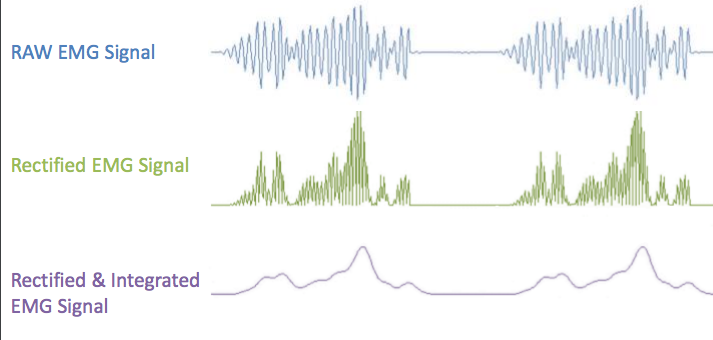
\includegraphics[scale=0.5]{EMGRect.png} $$

Therefore, we will either have to work with the raw data, or  we may need to do rectification and integration in live-time on our own.


\section{Background}


\begin{enumerate}


\item Reference pictures for forearm muscles:

$$ 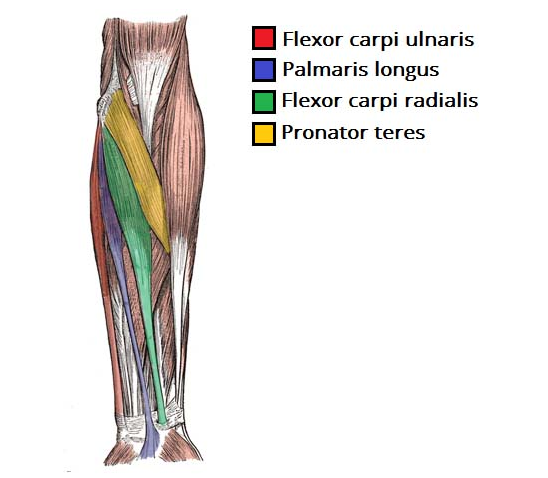
\includegraphics[scale = 0.3]{Forearm1.png}  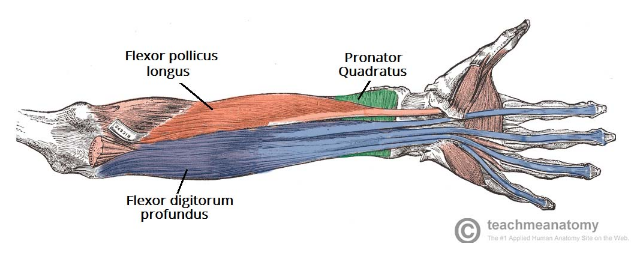
\includegraphics[scale =0.3]{Forearm2.png} $$

%TODO \href{}{blog} Link: http://teachmeanatomy.info/upper-limb/muscles/anterior-forearm/

Given the orientation of the EMG sensors, they will probably react well to flexion.  These diagrams will be useful for calibration purposes.



\item \textbf{N-Dimensional Dynamic Time Warping}


Dynamic Time Warping is a method by which to compare two time series with temporal differences. The following derivation is for N-Dimensional vectors in the time series. 

This is adapted from Gillian et al.

\vspace{5mm}

Let there be two N-dimensional time series, 

$$  \textbf{x} = \{ \vec{x}_1 ,  \vec{x}_2, ..  \vec{x}_{|\textbf{x}|} \}^T \   and \   \textbf{y} = \{    \vec{y}_1 ,  \vec{y}_2, ..  \vec{y}_{|\textbf{y}|}      \}^T $$, 

where each vector is of size N. 

We look to construct a warping path $ \textbf{w} = \{    \vec{w}_1 ,  \vec{w}_2, ..  \vec{w}_{|\textbf{w}|}      \}^T$ where the kth value of \textbf{w} 

$$ \vec{w}_k = ( \vec{x}_i , \vec{y}_j ) $$

is an $(\vec{x},\vec{y})$ pair chosen from their respective time series. The length, $ | \textbf{w} | $ is bounded by:

$$ max \{ | \textbf{x} |, | \textbf{y} | \} \leq | \textbf{w} | \leq | \textbf{x} | + | \textbf{y} | $$


In addition he warping path must adhere to the following constraints:

\begin{enumerate}

\item $w_1 = (1,1) $

\item $ w_{ | \textbf{w} |} =  ( | \textbf{x} |, | \textbf{y} | ) $

\item The warping path is continuous.

\item The warping path must be monotonic.

\end{enumerate}


In particular, we are looking for a warping path that gives the minimum normalized total warping distance between $ \textbf{x} $ and $ \textbf{y} $.

If we use a Euclidean metric to define the distance between any $ (\vec{x}, \vec{y}) $ as 

$$ DIST(\vec{x}, \vec{y}) = \sqrt{ \displaystyle \sum_{n=1}^N ( x(n) - y(n))^2 } $$

then the minimum normalized warping distance can be expressed as

$$ DTW( \textbf{x}, \textbf{y}) = \frac{1}{ | \textbf{w} | } \displaystyle \sum_{k=1}^{| \textbf{w} | }  DIST( \textbf{w}_{k_i},  \textbf{w}_{k_j} )) $$


The mininum total warping path can be found by using dynamic programing to fill a 2-D cost matrix, C, where each cell in the matrix represents the minimum warping cost to reach that point from the start. Under the rules given by our constraints, the cell value can be expressed by 


$$   C_{(i,j)} = DIST(i,j) + min ( C_{(i-1,j)} ,  C_{(i,j-1)} ,  C_{(i-1,j-1)}   )    $$ 


Once complete, we simply get the path by navigating the cost matrix in reverse order, as seen below:

$$ 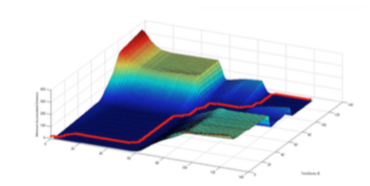
\includegraphics[scale =0.5]{DTW.png} $$


To train a template, we record $M_g$ training examples for each of the G gestures. The gth template can be found by searching for the training example that provides the minimum normalized total warping distance when matched agains the other $M_g -1 $ training examples in that class.  That is,

$$ \phi_g = arg min \ \ \frac{1}{M_g -1} \displaystyle \sum_{j=1}^{M_g}  DTW( \textbf{X}_i, \textbf{X}_j), \ \ \ \  1 \leq i \leq M_g,  i \neq j$$


To find the best therblig, we will simply get the the lowest cost from a comparison of the input with multiple time series, or output none if it doesn't reach a certain threshold.


$$  min \ \  DTW( \textbf{x}, \textbf{g})  $$ 

for each template $\textbf{g}$ in our set of gestures.

\vspace{5mm}


Nick Gillian's C++ Gesture Recognition Library has an implemetation of DTW.



\item Hand Activity Level 

The Akkas paper offered a method of quantizing the Hand Activity Level by fitting a linear regression equation as a function of root mean square (RMS) hand speed and duty cycle. In their work, hand speed is measured via  examination comparison of pixel windows featuring the region of interest (hand).  HAL expressed linearly was:

$$ HAL_{lin} = b_0 + b_1*S + b_2D  $$





To scale from 0 to 10, they used the following sigmoidal logit-linear regression:

$$    ln \ \  [  \frac{ \frac{HAL}{10}       }{  1 - \frac{HAL}{10}       }          ]  =     b_0 + b_1ln(S) + b_2D $$

solving, we get the following expression for HAL


$$ HAL_{log} = 10 [     \frac{e^{ b_0 + b_1ln(S) + b_2D}}{ 1 + e^{ b_0 + b_1ln(S) + b_2D}}       ]   $$



For the coefficients, $b_0 = -15.87, b_1 = 2.25,b_2 = 0.02$, they achieved a $R^2$ of 0.97. 

Below are the predicted HAL levels from the regression:

$$ 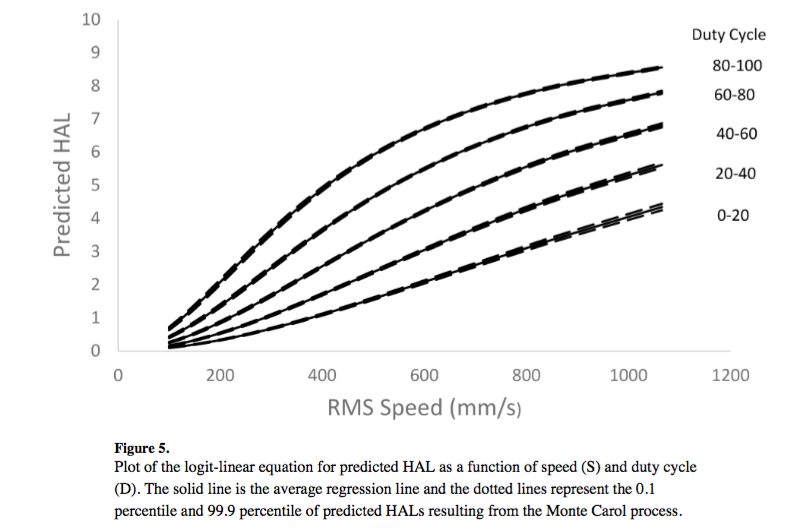
\includegraphics[scale=0.5]{HAL.png} $$



\end{enumerate}



\section{Planning - Therblig Recognition}


\subsection*{ a) Calibration}

The current implementation is to apply the Gesture Recognition Toolbox implementation of DTW to the raw EMG sensor output. This is not extendable for the following reasons:

Below is a label image of the EMG sensors. 

$$ 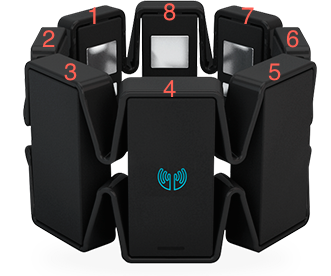
\includegraphics[scale=0.5]{EMGLabels.png} $$

We can see that the indexing is fixed relative to itself. Therefore the armband would have to go on the arm in the exact, discrete placement each time, and also have to read equivalently across all people's arms. DTW, which only handles temporal shifts in the data, would not be able to handle this type of variance.  

An ideal scenario would be that the individual user would be able to calibrate their input per trial, since we can expect the armband placement to be highly variable between trials, and the EMG readout to be distinct across different people. Calibration would allow us to standardize the input for comparison to the training set configured for the DTW algorithm.

I tentatively propose two calibration schemes, one for orientation and one for EMG normalization. 

\begin{enumerate}

\item Orientation - It is possible we can calibrate this by having the user open and close their hand repeatedly. We could expect to see a gradient of EMG values from the \textit{Flexor carpi ulnaris} to the \textit{Pronator teres}. This would give us the relative position of each EMG sensor in the unit circle around the arm.

$$ 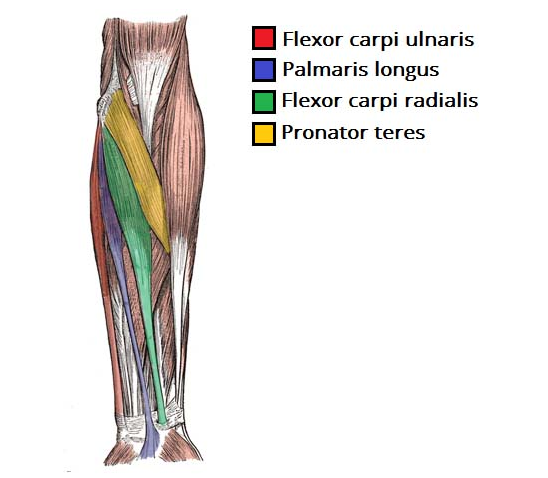
\includegraphics[scale = 0.3]{Forearm1.png} $$


Unfortunately, the EMG values are discrete and the armband expandable, and so there might be a slight shift on the exact position of the EMG sensor from trial to trial. If we can identify a maxima on the forearm, perhaps we can use interpolation to give us an interpolated value of the EMG at set coordinates and the exact location of the actual EMG sensors.


\item Normalization - if we can observe the interpolated maximum EMG value during the orientation phase, we could divide all values by this for a normalized input into the DTW algorithm.



\end{enumerate}


\subsection*{ b) Learning }

The following Therbligs are listed as Physical:

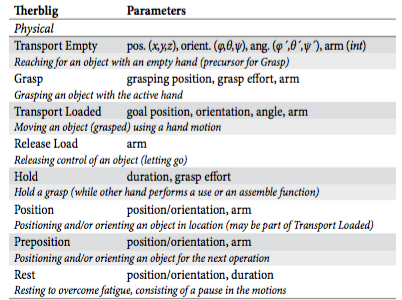
\includegraphics[scale = 0.75]{Therbligs.png}
 
The current code is training for the therbligs: Transport Empty, Grasp, and Transport Load.


Arguably, only Grasp and Release Load would have distinct DTW values. 


Hold and Transport Loaded would share the same DTW value, distinguished from each other by the absense or presence of accelerometer values. 

The same applies for Transport Empty and Rest. We would exect only to see a change in acceleration value, not EMG value.

The following questions remain:

\begin{enumerate}

\item Which therbligs are vital to identify, and which ones should be identified using DTW?

\item How do we identify a real-time time series window to feed into the DTW algorithm?

\end{enumerate}



\section{Planning - Hand Activity Level}

%TODO

From the current code, it seems that the current method is calculating the moving average of the acceleration and using it to update the velocity. This value is then fed into the equations with the given values from the regression fitting given above..

A moving average was probably used to accomodate due to raw acceleration output from the sensor.

Further work(?):

This might be working - I have not yet had the chance to setup and test it. How does this fit into the bigger picture? 




\end{document}